%!TEX TS-program = pdflatex
%!TEX TS-options = -shell-escape
%!TEX root = trajectory-grouping.tex
% -- Author: Jannes Bantje, j.bantje@wwu.de
\documentclass[a4paper,index=totoc,toc=bibliography,fontsize=11pt,DIV=13,headinclude,BCOR=5mm,cleardoublepage=empty,ngerman,draft]{scrreprt}
\usepackage{scrpage2} % wie fancyhdr, nur optimiert auf KOMA-Skript, leicht andere Syntax
\usepackage{etoolbox,letltxmacro} % zum Programmieren
\usepackage[final]{graphicx}
\robustify\rotatebox

% -- Farben
\usepackage[x11names]{xcolor}
\definecolor{dark_gray}{gray}{0.45}
\definecolor{light_gray}{gray}{0.6}
\definecolor{fb10_blue}{cmyk}{0.8,0.4,0.13,0.07}

\usepackage[utf8]{inputenc}
\usepackage[T1]{fontenc}
\usepackage{mathtools} % beinhaltet amsmath
\mathtoolsset{centercolon,showmanualtags}
\newtagform{brackets}{[}{]}
\usetagform{brackets}
\usepackage{fix-cm}
\usepackage[bbgreekl]{mathbbol}
\usepackage{amssymb} % zusätzliche Symbole
\usepackage{nicefrac} % schräge Brüche
\usepackage{faktor}
\newcommand{\Faktor}[1]{\faktor[\textstyle]{#1}}
\usepackage{xfrac}
\usepackage{cancel}
\usepackage{mathdots} % Verbesserung von Punkten wie zB \ldots
\usepackage[bb=px]{mathalfa}
\usepackage{centernot}

\usepackage{silence}
\WarningFilter{latexfont}{Size substitutions with differences}
\WarningFilter{latexfont}{Font shape `U/bbold/m/n' in size}

%!TEX root = trajectory-grouping.tex

% -- Zum Finetuning von Befehlen
\makeatletter
\newcommand{\raisemath}[1]{\mathpalette{\raisem@th{#1}}}
\newcommand{\raisem@th}[3]{\raisebox{#1}{$#2#3$}}
\makeatother

% -- Box mit vorgegebener minimaler Länge
\DeclareRobustCommand{\minwidthbox}[2]{%
  \ifmmode
    \expandafter\mathmakebox
  \else
    \expandafter\makebox
  \fi
  [\ifdim#2<\width\width\else#2\fi]{#1}%
}

% -- farbiges Untersteichen im Mathe-Modus
\def\mathul#1#2{\color{#1}\underline{{\color{black}#2}}\color{black}} 


% -- besserer underbrace befehl
\newcommand{\Underbrace}[2]{{\underbrace{#1}_{#2}}}





%--Mengen
\newcommand\SetSymbol[1][]{\nonscript\:#1\vert\allowbreak\nonscript\:\mathopen{}}
\providecommand\given{} % to make it exist
\DeclarePairedDelimiterX\set[1]\{\}{\renewcommand\given{\SetSymbol[\delimsize]}#1}

% -- Betrag und Skalarprodukt
\DeclarePairedDelimiter{\abs}{\lvert}{\rvert}
\DeclarePairedDelimiterX\skal[2]{\langle}{\rangle}{#1\,,\,#2}

%--Umklammern
\DeclarePairedDelimiter\enbrace{(}{)}
\DeclarePairedDelimiter\benbrace{[}{]}
\DeclarePairedDelimiter\homo{\llbracket}{\rrbracket}
\newcommand{\ssbrace}[1]{{\scriptscriptstyle\enbrace{#1}}}

%--Norm
\DeclarePairedDelimiter\norm{\Vert}{\Vert}






% - verbessertes Integral
\newcommand{\Int}[1]{\int_{\mathrlap{#1}}\,\,}

% -- Alles spezielles aus der Differentialtopologie
\newcommand{\Tang}{\ensuremath{\mathrm{T}\mkern-0.85mu}}
\newcommand{\mathd}{\ensuremath{\mathrm{d}\mkern-0.7mu}}
\newcommand{\diff}[2]{\ensuremath{\frac{{\partial #1}}{{\partial #2}}}}
\newcommand{\diffs}[2]{\ensuremath{\partial #1/\partial #2}}
\newcommand{\diffd}[2]{\ensuremath{\frac{\mathd #1}{\mathd #2} }}
\DeclareMathOperator{\Lie}{L}
\DeclareMathOperator{\Ad}{Ad}  
\DeclareMathOperator{\ad}{ad}
\DeclareMathOperator{\Spin}{Spin}
% \DeclareMathOperator{\spin}{spin}
\newcommand{\spin}{\mathop{\mathfrak{spin}}}
\newcommand{\Ce}{\mathcal{C}}
\DeclareMathOperator{\vol}{vol}



%--Abbildungsdefinition
\newcommand{\mapdef}[5]{%
	\[
		\begin{array}{rcl}
			\textstyle #1 &\xrightarrow{\minwidthbox{#5}{2em}} & \textstyle #2 \\[0.5ex]
			\textstyle #3 &\xmapsto{\minwidthbox{\mbox{ }}{2em}} & \textstyle #4
		\end{array}
	\]
}

%--modifiziertes Stackrel
\newcommand{\StackText}[2]{\stackrel{\mbox{\scriptsize #1}}{#2}}
\newcommand{\StackTextClap}[2]{\stackrel{\mathclap{\mbox{\scriptsize #1}}}{#2}}



 % Liste mit Mathebefehlen laden

% -- TikZ-Kram
\usepackage{tikz-cd}
\usetikzlibrary{quotes,babel,arrows.meta}
\tikzset{>=Straight Barb[]}
\tikzcdset{arrow style=math font}

% -- tikz/externalize
\usetikzlibrary{external}
\tikzexternalize[prefix=Bilder/tikz/, up to date check=diff]
\tikzset{external/system call={xelatex \tikzexternalcheckshellescape %-- verwende LuaLaTeX, wegen dynamischer Speicherallokation
    -halt-on-error -interaction=batchmode -jobname "\image" "\texsource"}}
\AtBeginEnvironment{tikzcd}{\tikzexternaldisable}
\AtEndEnvironment{tikzcd}{\tikzexternalenable}
\pgfkeys{/pgf/images/include external/.code=\includegraphics{#1}}

% -- Einstellungen bezüglich Schriftart etc.
\usepackage{ccfonts}
\usepackage[semibold]{sourcesanspro}
\usepackage[semibold,scale=.95]{sourcecodepro}
\usepackage{eulervm}

% \addtokomafont{disposition}{\sffamily}

\usepackage{fontawesome}
\usepackage[final]{microtype}
\flushbottom
\KOMAoptions{DIV=last}


% -- Einstellungen bezüglich der Sprache, Silbentrennung etc.
\usepackage{babel}
% \usepackage{polyglossia}
% \setmainlanguage[spelling=new,babelshorthands=true]{german}
% \setotherlanguage[variant=british]{english}

% -- BibLaTeX 
\usepackage[%
	backend=biber,
	sortlocale=auto,
	natbib,
	hyperref,
	backref,
	style=alphabetic
	]%
{biblatex}
\renewcommand*{\mkbibnamelast}[1]{%
  \ifmknamesc{\textsc{#1}}{#1}}

\renewcommand*{\mkbibnameprefix}[1]{%
  \ifboolexpr{ test {\ifmknamesc} and test {\ifuseprefix} }
    {\textsc{#1}}
    {#1}}

\def\ifmknamesc{%
  \ifboolexpr{ test {\ifcurrentname{labelname}}
               or test {\ifcurrentname{author}}
               or ( test {\ifnameundef{author}} and test {\ifcurrentname{editor}} ) }}
\addbibresource{quellen.bib}

% -- Konfiguration von Hyperref
\usepackage[hidelinks, pdfpagelabels, bookmarksopen=true, bookmarksnumbered=true, linkcolor=black, urlcolor=SkyBlue2, plainpages=false,pagebackref, citecolor=black, hypertexnames=true, pdfauthor={Jannes Bantje}, pdfborderstyle={/S/U}, linkbordercolor=SkyBlue2, colorlinks=false,backref=false]{hyperref}
\hypersetup{final}

\usepackage[nameinlink,noabbrev]{cleveref}

% -- \url aufhübschen
\newcommand{\appendLink}[1]{#1\,\faExternalLink}
\newcommand{\hrefsym}[2]{\href{#1}{\texttt{\appendLink{#2}}}}
\renewcommand{\url}[1]{\hrefsym{#1}{\nolinkurl{#1}}}

% -- Aufzählungen, Anführungszeichen etc.
\usepackage[shortlabels,inline]{enumitem}
\setlist[itemize,1]{label=\scriptsize$\blacksquare$}
\usepackage[autostyle,german=quotes]{csquotes}


% -- Indexverarbeitung
\usepackage{makeidx}
\newcommand{\bet}[1]{\emph{#1}}
\newcommand{\Index}[1]{\bet{#1}\index{#1}}
\makeindex
% \setindexpreamble{{\noindent \itshape Die Seitenzahlen sind mit Hyperlinks zu den entsprechenden Seiten versehen, also anklickbar}\par \bigskip}
\renewcommand{\indexpagestyle}{scrheadings}

% -- Alles zum Thema Gliederung
% \usepackage{chngcntr}
% \counterwithin*{equation}{section}
\numberwithin{equation}{section}
% \setcounter{tocdepth}{3}

% -- theorem packages
\let\openbox\relax
\usepackage{amsthm}
\usepackage{thmtools,thm-restate}
\usepackage{mdframed}
\renewcommand{\listtheoremname}{Übersicht aller Aussagen}

% -- Theoreme als PDF-Lesezeichen
\usepackage{bookmark}
\bookmarksetup{open,numbered}
\makeatletter
\newcommand*{\theorembookmark}{%
  \bookmark[
    dest=\@currentHref,
    rellevel=1,
    keeplevel,
  ]{%
    \thmt@thmname\space\csname the\thmt@envname\endcsname
    \ifx\thmt@shortoptarg\@empty
    \else
      \space(\thmt@shortoptarg)%
    \fi
  }%
}   
\makeatother

% -- Definition der einzelnen Umgebungen
\declaretheoremstyle[%
	headfont=\sffamily\bfseries,
	notefont=\normalfont\sffamily,
	bodyfont=\normalfont,
	headformat=\NUMBER\ \NAME\NOTE,
	headpunct=.,
	postheadspace=1em,
	spaceabove=15pt,spacebelow=10pt,
	shaded={bgcolor=gray!20},
	% mdframed={%
	% 	backgroundcolor=gray!20,
	% 	innertopmargin=0pt,
	% 	innerleftmargin=0pt,
	% 	% roundcorner=5pt,
	% 	innerbottommargin=0pt,
	% 	splittopskip = 0pt,
	% 	% skipbelow=6pt,
	% 	% skipbelow=6pt,
	% 	topline=false,bottomline=false,leftline=false,rightline=false
	% },
	postheadhook=\theorembookmark]%
{mainstyle}
\declaretheoremstyle[%
	headfont=\sffamily\bfseries,
	notefont=\normalfont\sffamily,
	bodyfont=\normalfont,
	headformat=\NUMBER\ \NAME\NOTE,
	headpunct=.,
	postheadspace=1em,
	spaceabove=15pt,spacebelow=10pt,
	shaded={bgcolor=fb10_blue!20},
	postheadhook=\theorembookmark]%
{mainstyle_blue}
\declaretheoremstyle[%
	headfont=\sffamily\bfseries,
	notefont=\normalfont\sffamily,
	bodyfont=\normalfont,
	headformat=\NUMBER\ \NAME\NOTE,
	headpunct=.,
	postheadspace=1em,
	spaceabove=15pt,spacebelow=10pt,
	postheadhook=\theorembookmark]%
{mainstyle_unshaded}
\declaretheoremstyle[%
	headfont=\sffamily\bfseries,
	notefont=\normalfont\sffamily,
	bodyfont=\normalfont,
	headformat=\NUMBER\NAME\NOTE,
	headpunct=.,
	postheadspace=1em,
	spaceabove=15pt,spacebelow=10pt,
	% shaded={bgcolor=gray!20},
	postheadhook=\theorembookmark]%
{mainstyle_unnumbered}
\declaretheoremstyle[%
	headfont=\sffamily\bfseries,
	notefont=\normalfont\sffamily,
	bodyfont=\normalfont,
	headformat=swapnumber,
	headpunct=.,
	postheadspace=1em,
	spaceabove=15pt,spacebelow=10pt,
	shaded={bgcolor=gray!20},
	postheadhook=\theorembookmark,
	qed=\qedsymbol]%
{mainstyleB}
\declaretheorem[name=Definition,parent=section,style=mainstyle_blue]{definition}
\declaretheorem[name=Definition \& Proposition,refname=Proposition,sharenumber=definition,style=mainstyle_blue]{definitionP}
\declaretheorem[name=Definition,numbered=no,style=mainstyle_unnumbered]{definition*}
\declaretheorem[name=Theorem,sharenumber=definition,style=mainstyle]{theorem}
\declaretheorem[name=Theorem,numbered=no,style=mainstyle_unnumbered]{theorem*}
\declaretheorem[name=Proposition,sharenumber=definition,style=mainstyle,refname=Proposition]{proposition}
\declaretheorem[name=Lemma,sharenumber=definition,style=mainstyle]{lemma}
\declaretheorem[name=Satz,refname=Satz,sharenumber=definition,style=mainstyle]{satz}
\declaretheorem[name=Satz,sharenumber=definition,style=mainstyle_unshaded]{satzUnshaded}
\declaretheorem[name=Definition,sharenumber=definition,style=mainstyle_unshaded]{definitionUnshaded}
\declaretheorem[name=Satz,numbered=no,style=mainstyle_unnumbered]{satz*}
\declaretheorem[name=Korollar,sharenumber=definition,style=mainstyle]{korollar}
\declaretheorem[name=Korollar,sharenumber=definition,style=mainstyleB]{korollarB}
\declaretheorem[name=Frage,numbered=no,style=mainstyle_unnumbered]{frage}
\declaretheorem[name=Frage,sharenumber=definition,style=mainstyle_unshaded]{frageA}
\declaretheorem[name=Erinnerung,sharenumber=definition,style=mainstyle_unshaded]{erinnerungA}
\declaretheorem[name=Ausblick,sharenumber=definition,style=mainstyle_unshaded]{ausblick}
\declaretheorem[name=Konvention,sharenumber=definition,style=mainstyle]{konvention}
\declaretheorem[name=Notation,sharenumber=definition,style=mainstyle_unshaded]{notation}
\declaretheorem[name=Bemerkung,sharenumber=definition,style=mainstyle_unshaded]{bemerkung}
\declaretheorem[name=Bemerkung,numbered=no,style=mainstyle_unnumbered]{bemerkung*}
\declaretheorem[name=Beispiel,sharenumber=definition,style=mainstyle_unshaded]{beispiel}
\declaretheorem[name=Beispiel,numbered=no,style=mainstyle_unnumbered]{beispiel*}
\declaretheorem[name=Exkurs,numbered=no,style=mainstyle_unnumbered]{exkurs*}

% english versions
\declaretheorem[name=Remark,sharenumber=definition,style=mainstyle_unshaded]{remark}
\declaretheorem[name=Remark,numbered=no,style=mainstyle_unnumbered]{remark*}
\declaretheorem[name=Example,sharenumber=definition,style=mainstyle_unshaded]{example}
\declaretheorem[name=Corollary,sharenumber=definition,style=mainstyle]{corollary}

% -- Beweise
\declaretheoremstyle[headfont=\bfseries\scshape,bodyfont=\normalfont,headpunct=:,postheadspace=1em,spacebelow=12pt,spaceabove=2pt,qed=\qedsymbol]{beweise}
\declaretheoremstyle[headfont=\bfseries\scshape,bodyfont=\normalfont,headpunct=:,postheadspace=1em,spacebelow=12pt,spaceabove=2pt]{beweisskizze}
\declaretheoremstyle[headfont=\sffamily\bfseries,bodyfont=\normalfont,headpunct=:,postheadspace=1em,spacebelow=10pt,spaceabove=10pt]{bemerkungen}
\declaretheorem[name=Beweis,numbered=no,style=beweise]{beweis}
\let\proof\relax
\declaretheorem[name=Proof,numbered=no,style=beweise]{proof}
\declaretheorem[name=Sketch of Proof,numbered=no,style=beweisskizze]{sketch}

\declaretheorem[name=Übung,numbered=no,style=bemerkungen]{uebung}
\declaretheorem[name=Erinnerung,numbered=no,style=bemerkungen]{erinnerung}


% -- marginnotes package
\usepackage[fulladjust]{marginnote}
\renewcommand*{\marginfont}{\itshape \footnotesize}
\usepackage{ragged2e}
\renewcommand*{\raggedleftmarginnote}{\RaggedLeft}
\renewcommand*{\raggedrightmarginnote}{\RaggedRight}

% -- todonotes package
\usepackage[textsize=small,obeyDraft]{todonotes}
\LetLtxMacro{\oldtodo}{\todo}
\renewcommand{\todo}[2][]{\tikzexternaldisable\oldtodo[#1]{#2}\tikzexternalenable}
\LetLtxMacro{\oldmissingfigure}{\missingfigure}
\renewcommand{\missingfigure}[2][]{\tikzexternaldisable\oldmissingfigure[{#1}]{#2}\tikzexternalenable}

% -- Fußnoten anpassen
\deffootnote[1.5em]{1.5em}{1.5em}{\textsuperscript{\thefootnotemark}\ }

% -- Figures und Captions
\usepackage{wrapfig}

%--Römische Zahlen
\newcommand{\RM}[1]{\MakeUppercase{\expandafter{\romannumeral #1.\relax}}}
\robustify\RM


% -- Metadaten für die Titelei
\author{Jannes Bantje}


% -- Kopf- und Fußzeilen
\setheadsepline{1pt}[\color{light_gray}]
\pagestyle{scrheadings}
\clearscrheadfoot
\automark{section}
\lehead{
\includegraphics[height=0.6 cm,keepaspectratio]{Bilder/Logo_WWU_Muenster_light_gray.pdf}}
\lohead{\color{dark_gray}\normalfont\footnotesize\sffamily\itshape Gruppierung von Trajektorien -- Seminarvortrag von Jannes Bantje}
\rohead{
\includegraphics[height=0.6 cm,keepaspectratio]{Bilder/fb10logo_gray.pdf}}

\ofoot[{\color{dark_gray}\sffamily\LARGE \thepage}]{{\color{dark_gray}\sffamily\LARGE \thepage}} %hier wir auch der plain Stil bearbeitet!
\ifoot{ \color{dark_gray} \sffamily\small \leftmark}

% -- Inhaltsverzeichnis und weitere Pakte, die zuletzt geladen werden sollten
\usepackage[tocindentauto]{tocstyle}
\usetocstyle{KOMAlike}
\usepackage{ellipsis}



\begin{document}
\pagenumbering{Roman}

%!TEX root = trajectory-grouping.tex
\begin{titlepage}
\hspace*{0.12\textwidth}% Whitespace to the left of the title page
\rule{2pt}{\textheight}% Vertical line
\hspace*{0.05\textwidth}% Whitespace between the vertical line and title page text
\begin{minipage}[b]{0.80\textwidth}
	\raggedright
	
\includegraphics[height=1.5cm, keepaspectratio]{Bilder/Logo_WWU_Muenster.pdf} \\[2cm]
	{\Large \sffamily Ausarbeitung zum Seminarvortrag}\\[0.5cm]
	{\Huge\sffamily\bfseries Gruppierung von Trajektorien}\\[.5cm]
	{\large\sffamily basierend auf \citetitle{buchin2015} von \citeauthor{buchin2015}}\\[5cm]
	{\large \textit{Autor:}}\\[5pt]
	{\Large \textsc{Jannes Bantje}}\\[5pt] % Author name
	{\small\email{j.bantje@wwu.de}\\ Matr.\,Nr.: 395\,197}\\[2.5cm]
	
	\vspace{0.1\textheight}
	
\includegraphics[height=1cm, keepaspectratio]{Bilder/fb10logo.pdf}
	% \hfill\includegraphics[height=8cm,keepaspectratio]{Bilder/E8_graph.pdf}
\end{minipage}	


% \begin{center}
% \vspace*{10cm}
% \includegraphics[height=9cm,keepaspectratio]{Bilder/E8_graph.pdf}
% \end{center}

\end{titlepage}

\tableofcontents

\section*{Notation}
\addcontentsline{toc}{section}{Notation}
Im Verlauf dieser Arbeit gelten die folgenden Konventionen
\begin{itemize}
	\item 
\end{itemize}
Das Vorgehen richtet sich in erster Linie nach \textcite{buchin2015}.
\cleardoubleoddemptypage
\pagenumbering{arabic}
\setcounter{page}{1}
\setcounter{footnote}{0}

\chapter{Einleitung und Problemstellung} % (fold)
\label{cha:einleitung}
%!TEX root = ../trajectory-grouping.tex
Betrachtet man eine Menge von sich bewegenden Entitäten, so haben wir bereits im dritten Beitrag dieses Seminars festgestellt, dass für die Analyse solcher Daten eine Gruppierung einzelner Trajektorien äußerst nützlich ist.
In diesem Beitrag soll eine solche Gruppierung mit Methoden der Topologie erläutert werden.\todo{Kapitel aus Buch durchlesen, um Unterschiede betonen zu können}

Intuitiv soll eine Menge ausreichend vieler sich bewegender Entitäten, die sich für eine gewisse Zeit lang \enquote{zusammen bewegen}, eine Gruppe bilden.
Unsere erste Aufgabe wird es sein, diese Intuition in eine mathematische Definition zu überführen.
Diese intuitive Definition suggeriert bereits, dass dabei drei Parameter in eine Definition mit eingehen sollten:
\begin{description}
	\item[Mindestgröße] Auch wenn man prinzipiell den Fall einer einelementigen Gruppe betrachten kann, sollte eine Gruppe im Allgemeinen eine gewisse Mindestgröße haben, die sich gegebenenfalls aus dem Anwendungsfall ergibt, oftmals aber auch während der Analyse variiert wird.
	So gelangt man zu einer detaillierten Sicht auf Gruppierungen, wenn man die Mindestgröße verringert, da so mehr Gruppen entstehen.
	\item[Dauer/zeitlicher Parameter] Entitäten, die sich nur kurz \enquote{begegnen}, aber nicht zusammen bewegen, sollten nicht unbedingt zu einer Gruppe zusammengefasst werden, was durch die Forderung einer minimalen Dauer der gemeinsamen Bewegung gewährleistet wird.
	Auch hier erhält man eine detailliertere Sicht auf Gruppierungen, wenn man die minimale Dauer geringer ansetzt, da dann tendenziell mehr Gruppen entstehen.
	\item[Räumlicher Parameter] Um von einer gemeinsamen Bewegung sprechen zu können, dürfen die Entitäten offensichtlich nicht zu weit voneinander entfernt sein und wir benötigen einen Parameter für den Abstand zwischen den Entitäten.
	Hier erhalten wir eine detailliertere Sicht mit mehr Gruppen durch Vergrößerung dieses Parameters.
\end{description}
Diese drei Parameter ermöglichen es uns, Gruppierungen in verschiedenen Größenordnungen zu analysieren und unser Augenmerk auf bestimmte Gruppen zu lenken: Bei einer hohen Mindestgröße interessieren wir uns nur für große Gruppen, wählen wir einen großen zeitlichen Parameter, so betrachten wir lediglich lange bestehende Gruppen und ein kleiner räumlicher Parameter filtert lose zusammenhängende Gruppen heraus.

Das hier vorgestellte Modell leistet aber noch deutlich mehr als die Identifikation der Gruppen, den es beinhaltet auch die Veränderungen der \GrpStruktur über den betrachteten Zeitraum.
Insbesondere werden neben \emph{Start}- und \emph{End}-Ereignissen auch \emph{Merge}- und \emph{Split}-Ereignisse beachtet, das heißt es lässt sich eine detaillierte Historie der \GrpStruktur erstellen.

Bevor wir im folgenden \cref{cha:def_gruppe} Gruppen mathematisch präzise definieren, soll hier noch das Zusammenspiel der Parameter an möglichen Anwendungsgebieten demonstriert werden.
\todo[inline]{mögliche Anwendungsgebiete}
% chapter einleitung (end)

\chapter{Definition einer Gruppe von Trajektorien} % (fold)
\label{cha:def_gruppe}
%!TEX root = ../trajectory-grouping.tex

Wir bezeichnen mit $\mathcal{X}$ die Menge der Entitäten, zu denen uns der Ort innerhalb eines gewissen Zeitraums bekannt ist.
Wie in \cref{cha:einleitung} angedeutet wird unsere Definition einer Gruppe von den folgenden drei Parametern abhängen, die Charakteristika der zu betrachtenden Gruppen bestimmen:
\begin{itemize}
	\item Räumlicher Parameter $\varepsilon > 0$
	\item zeitlicher Parameter $\delta > 0$
	\item Mindestgröße $m \in \mathbb{N}\setminus \set*{0}$
\end{itemize}
Wir beginnen mit einigen Definitionen zum räumlichen Zusammenhang zu einem festen Zeitpunkt $t$.\todo{Scheibe offen oder geschlossen?}
\begin{definition}
	Die $\varepsilon$-Scheibe $B_\varepsilon^t(x)$ einer Entität $x$ zum Zeitpunkt $t$ ist eine Scheibe mit Radius $\varepsilon$ um $x$ zu Zeitpunkt $t$, also $B_\varepsilon^t(x) = \set*{y \in \mathbb{R}^d \given \norm*{x^t-y} \le \varepsilon}$.\marginnote{wir betrachten meist $d=2$}
	
	Zwei Entitäten $x$ und $y$ sind zum Zeitpunkt $t$ \Index{direkt zusammenhängend}, falls sich die $\varepsilon$-Scheiben überlappen, das heißt der Schnitt der beiden offenen Scheiben nicht leer ist.
	
	Die Entitäten $x$ und $y$ heißen \bet{$\varepsilon$-zusammenhängend}\index{epsilon-zusammenhängend@$\varepsilon$-zusammenhängend} zum Zeitpunkt $t$, falls eine Folge von Entitäten $x=x_0, \ldots, x_k = y$ existiert, sodass $x_i$ und $x_{i+1}$ direkt zusammenhängend sind.
\end{definition}

Eine Teilmenge $\mathcal{S} \subseteq \mathcal{X}$ heißt dementsprechend \bet{$\varepsilon$-zusammenhängend}, falls alle Entitäten in $\mathcal{S}$ paarweise $\varepsilon$-zusammenhängend sind.
Dies ist äquivalent dazu, dass das Innere der Vereinigung aller $\varepsilon$-Scheiben der Entitäten von $\mathcal{S}$ zusammenhängend ist.
Wir nennen $\mathcal{S}$ eine \Index{Komponente} zum Zeitpunkt $t$, falls $\mathcal{S}$ eine maximale $\varepsilon$-zusammenhängende Teilmenge ist.
Die Menge der Komponenten zum Zeitpunkt $t$ bezeichnen wir mit $\mathcal{C}(t)$; sie bildet eine Partition von $\mathcal{X}$ zum Zeitpunkt $t$.

\Cref{fig:components} zeigt die Auswirkung verschiedener $\varepsilon$-Werte auf die Partition der Entitäten in verschiedene $\varepsilon$-Komponenten.

\begin{figure}[bthp]
	\Centering
	\subfloat[Mit $\varepsilon=\SI{0.4}{\centi\metre}$ liegen alle Punkte in einer Komponente]{
		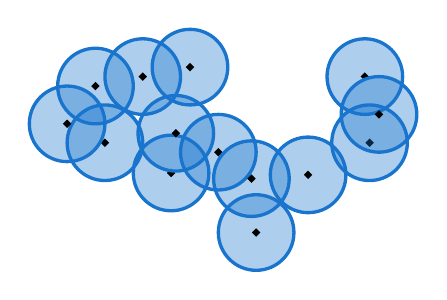
\begin{tikzpicture}[scale=1.2]
			% \draw[help lines] (-1,-1) grid (2,2);
			\coordinate (1) at (0,-0.02);
			\coordinate (2) at (.05,.4);
			\coordinate (3) at (.5,.2);
			\coordinate (4) at (.85,-.08);
			\coordinate (5) at (1.45,-.04);
			\coordinate (6) at (-0.7,.3);
			\coordinate (7) at (2.1,.3);
			\coordinate (8) at (2.05,1);
			\coordinate (9) at (0.2,1.1);
			\coordinate (10) at (.9,-.65);
			\coordinate (11) at (2.2,.6);
			\coordinate (12) at (-.3,1);
			\coordinate (13) at (-.8,.9);
			\coordinate (14) at (-1.1,.5);
			\foreach \x in {1,2,...,14}{
				\draw[DodgerBlue3,fill=DodgerBlue3,fill opacity=.35,very thick] (\x) circle[radius=.4];
				\draw[fill,very thick] (\x) circle[radius=.02];
			}
		\end{tikzpicture}
	}
	\hspace{2cm}
	\subfloat[Mit $\varepsilon=\SI{0.3}{\centi\metre}$ erhält man drei Komponenten]{
		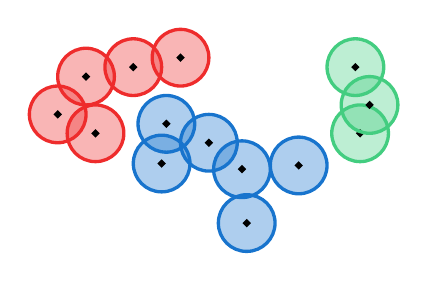
\begin{tikzpicture}[scale=1.2]
			% \draw[help lines] (-1,-1) grid (2,2);
			\coordinate (1) at (0,-0.02);
			\coordinate (2) at (.05,.4);
			\coordinate (3) at (.5,.2);
			\coordinate (4) at (.85,-.08);
			\coordinate (5) at (1.45,-.04);
			\coordinate (6) at (-0.7,.3);
			\coordinate (7) at (2.1,.3);
			\coordinate (8) at (2.05,1);
			\coordinate (9) at (0.2,1.1);
			\coordinate (10) at (.9,-.65);
			\coordinate (11) at (2.2,.6);
			\coordinate (12) at (-.3,1);
			\coordinate (13) at (-.8,.9);
			\coordinate (14) at (-1.1,.5);
			\foreach \x in {1,2,...,5,10}{
				\draw[DodgerBlue3,fill=DodgerBlue3,fill opacity=.35,very thick] (\x) circle[radius=.3];
				\draw[fill,very thick] (\x) circle[radius=.02];
			}
			\foreach \x in {6,9,12,13,14}{
				\draw[Firebrick2,fill=Firebrick2,fill opacity=.35,very thick] (\x) circle[radius=.3];
				\draw[fill,very thick] (\x) circle[radius=.02];
			}
			\foreach \x in {7,8,11}{
				\draw[SeaGreen3,fill=SeaGreen3,fill opacity=.35,very thick] (\x) circle[radius=.3];
				\draw[fill,very thick] (\x) circle[radius=.02];
			}
		\end{tikzpicture}
	}
	\caption{Komponenten einer 14-elementigen Punktmenge zu verschiedenen $\varepsilon$-Werten}\label{fig:components}
\end{figure}

\begin{definition}[{name=[Gruppe während eines Zeitraums]}]
	Eine Menge $G$ von $k$ Entitäten bildet eine \Index{Gruppe} im Zeitintervall $I$, falls folgendes gilt:
	\begin{enumerate}[(i)]
		\item $G$ enthält mindestens $m$ Entitäten, also $k \ge m$
		\item die Länge von $I$ ist mindestens $\delta$
		\item zu jeder Zeit $t \in I$ existiert eine Komponente $C \in \mathcal{C}(t)$ mit $G \subseteq C$.
	\end{enumerate}
	Das Intervall $I=[t_s,t_e]$ der Gruppe $G$ bezeichnen wir auch mit $I_G$.
	Eine Gruppe $H$ \bet{überlagert}\index{Gruppe!überlagernde} $G$, falls $G \subseteq H$ und $I_G \subseteq I_H$ gilt.
	Falls kein solches $H$ existiert, so heißt $G$ \bet{maximal}\index{Gruppe!maximale}. 
\end{definition}

Da wir ja eigentlich die Trajektorien einzelner Entitäten gruppieren wollen, mag es auf den ersten Blick etwas kontraintuitiv erscheinen, dass eine Entität $x$ in mehreren maximalen Gruppen enthalten sein kann, da zum Überlagern auch die Inklusion der Zeitintervalle gegeben sein muss.

% chapter def_gruppe (end)

\chapter{Reeb-Graphen und Repräsentation der \GrpStruktur} % (fold)
\label{cha:reeb_graphen}
%!TEX root = ../trajectory-grouping.tex
Sei $X$ ein topologischer Raum und $f \colon X \to \mathbb{R}$ eine stetige Funktion.
Dann bezeichnet man für einen Wert $a \in \mathbb{R}$ das Urbild unter $f$ als \Index{Niveaumenge} (engl. \emph{level set}) von $a$.
Die Niveaumengen bilden offensichtlich eine Partition von $X$.

Anschaulich stellt man sich $f$ meist als \Index{Höhenfunktion} vor. 
So könnte $X$ beispielsweise das Gebiet einer Karte in einem handelsüblichen Atlas sein (=eine Teilmenge der zweidimensionalen Ebene) und $f$ gibt die Höhe über NN an.
Dann sind die Niveaumengen $f^{-1}(\set{a})$ genau die Niveaulinien, die man in detaillierten topografischen Karten findet (ein Beispiel einer solchen Karte findet sich in \cref{sec:karte_niveau}).

Um den \Index{Reeb-Graph} von $f$ zu erhalten, benutzen wir nun die Zusammenhangskomponenten von $f^{-1}(\set{a})$ wie folgt (Definition nach \textcite[\RM{6}.4]{compTopo})

\begin{definition}[{name=[Reeb-Graph]}]
	Der \Index{Reeb-Graph} zu $f \colon X \to \mathbb{R}$ ist der Quotientenraum $\mathcal{R}(f) \coloneqq X/{\sim}$ bezüglich der folgenden Äquivalenzrelation
	\[
		x \sim y \,:\mkern-3mu\iff \exists a \in \mathbb{R} : x,y \text{ liegen in der gleichen Zusammenhangskomponente von } f^{-1}(\set{a}) 
	\]
	Die Elemente von $\mathcal{R}(f)$ bezeichnen wir als \Index{Konturen} von $f$.
\end{definition}
Wir erhalten eine eindeutig bestimme Abbildung $h \colon \mathcal{R}(f) \to \mathbb{R}$, sodass das folgende Diagramm kommutiert.
Alle Abbildungen sind aufgrund der universellen Eigenschaft der Quotiententopologie stetig.
\[
	\begin{tikzcd}[sep=large]
		X \rar["f"] \dar["q",two heads] & \mathbb{R} \\
		\mathcal{R}(f) \urar["h"']
	\end{tikzcd}
\]
Die Quotientenabbildung $q$ bildet einen Punkt aus $X$ auf die zugehörige Kontur in $\mathcal{R}(f)$ ab.
$\mathcal{R}(f)$ ist tatsächlich ein Graph, da jede Niveaumenge unter $q$ auf eine diskrete Menge abgebildet wird.\todo{genauer bzw. expliziter}
Betrachtet man die positive Richtung in $\mathbb{R}$, so wird $\mathcal{R}(f)$ auf kanonische Weise zu einem gerichteten Graphen.

\section{Differentialtopologische Hintergründe zum Reeb-Graphen} % (fold)
\label{sec:background_reeb}
\begin{figure}[tbhp]
	\Centering
	\begin{tikzpicture}[rotate=90, xscale=1, yscale=1, scale=0.7]
		% \draw[help lines] (-4,-10) grid (4,4);
		% reelle Gerade
		\draw[->,thick] (-4,-6) -- ++ (8,0) node[left=3pt]{$\mathbb{R}$};
		
		\draw[DodgerBlue3, thick] (-2.5,1.89) .. controls +(240:0.8) and +(120:0.8) .. (-2.5,-1.89);
		\draw[DodgerBlue3, thick, dashed] (-2.5,1.89) .. controls +(300:0.8) and +(60:0.8) .. (-2.5,-1.89);
		\draw[fill=DodgerBlue3] (-2.5,-6) circle[radius=0.07];
		
		\draw[Firebrick2, thick] (0,2.5) .. controls +(250:0.6) and +(110:0.6) .. (0,0.5);
		\draw[Firebrick2, thick, dashed] (0,2.5) .. controls +(290:0.6) and +(70:0.6) .. (0,0.5);
		
		\draw[Firebrick2, thick] (0,-0.5) .. controls +(250:0.6) and +(110:0.6) .. (0,-2.5);
		\draw[Firebrick2, thick, dashed] (0,-0.5) .. controls +(290:0.6) and +(70:0.6) .. (0,-2.5);
		\draw[fill=Firebrick2] (0,-6) circle[radius=0.07];
		
		\draw[SeaGreen3, thick] (1.75,2.25) .. controls +(250:0.6) and +(110:0.6) .. (1.75,0) .. controls +(250:0.6) and +(110:0.6) .. (1.75,-2.25);
		\draw[SeaGreen3, thick, dashed] (1.75,2.25) .. controls +(290:0.6) and +(70:0.6) .. (1.75,0) .. controls +(290:0.6) and +(70:0.6) .. (1.75,-2.25);
		\draw[fill=SeaGreen3] (1.75,-6) circle[radius=0.07];
		
		\draw[SeaGreen3, thick] (-1.75,2.25) .. controls +(250:0.6) and +(110:0.6) .. (-1.75,0) .. controls +(250:0.6) and +(110:0.6) .. (-1.75,-2.25);
		\draw[SeaGreen3, thick, dashed] (-1.75,2.25) .. controls +(290:0.6) and +(70:0.6) .. (-1.75,0) .. controls +(290:0.6) and +(70:0.6) .. (-1.75,-2.25);
		\draw[fill=SeaGreen3] (-1.75,-6) circle[radius=0.07];
		
		% kritische Werte and Start und Ende
		\begin{scope}
			\clip (-3.5,-1) rectangle (3.5,1);
			\draw[Sienna2,fill=Sienna2] (3.5,0) circle[radius=.08];
			\draw[Sienna2,fill=Sienna2] (-3.5,0) circle[radius=.08];
		\end{scope}
		\draw[fill=Sienna2] (3.5,-6) circle[radius=.07];
		\draw[fill=Sienna2] (-3.5,-6) circle[radius=.07];
		
		% draw reeb graph
		\begin{scope}[every node/.style={shape=circle,inner sep=1.7pt,fill}]
			\draw[thick] (-3.5,-12) node{} -- ++(1.75,0) .. controls +(80:1.5) and +(100:1.5) .. ++(3.5,0) node{};
			\draw[thick] (3.5,-12) node{}-- ++(-1.75,0) .. controls +(-100:1.5) and +(-80:1.5) .. ++(-3.5,0) node{};
		\end{scope}
		\node at (3,-11) {$\mathcal{R}(f)$}; 
		
		\draw[thick] (-3.5,0) .. controls (-3.5,2) and (-1.5,2.5) .. (0,2.5);
		\draw[thick,xscale=-1] (-3.5,0) .. controls (-3.5,2) and (-1.5,2.5) .. (0,2.5);
		\draw[thick,rotate=180] (-3.5,0) .. controls (-3.5,2) and (-1.5,2.5) .. (0,2.5);
		\draw[thick,yscale=-1] (-3.5,0) .. controls (-3.5,2) and (-1.5,2.5) .. (0,2.5);
		\draw[thick] (-2,.2) .. controls (-1.5,-0.3) and (-1,-0.5) .. (0,-.5) .. controls (1,-0.5) and (1.5,-0.3) .. (2,0.2);
		\draw[thick] (-1.75,0) .. controls (-1.5,0.3) and (-1,0.5) .. (0,.5) .. controls (1,0.5) and (1.5,0.3) .. (1.75,0);
		
		\draw[-to] (0,-3.5) -- (0,-5) node[above, midway]{$f$};
	\end{tikzpicture}
	\caption[Höhenfunktion des aufrechten Torus mit dem dazugehörigen Reeb-Graphen]{Höhenfunktion des aufrechten Torus $T^2=S^1 \times S^1$ mit dem dazugehörigen Reeb-Graphen. Die grün und orange gekennzeichneten Niveaumengen enthalten je einen kritischen Punkt, die rote und blaue enthalten ausschließlich reguläre Werte. $f$ ist eine Morse-Funktion und die Knoten des Reeb-Graphen stehen in Bijektion zu den kritischen Punkten.}\label{fig:torus_reeb}
\end{figure}
Obwohl wir den Reeb-Graph allgemein definiert haben und auch im weiteren Verlauf keine differenzierbare Struktur auf $X$ benötigen, ist es an dieser Stelle sinnvoll einen kurzen Ausflug in die Differentialtopologie zu machen, um mit einem instruktiven Beispiel zu erläutern, wo genau die Knoten im Reeb-Graphen \enquote{herkommen}.
Neben den gleich auch direkt referenzierten Büchern von \textcite{compTopo} und \textcite{MilnorMorse}, sei an dieser Stelle auf das Buch \citetitle{Miln} von \textcite{Miln} verwiesen, welches einen schnellen, lesenswerten Einstieg in die Grundlagen der Differentialtopologie vermittelt.

Betrachtet man nicht einen beliebigen topologischen Raum $X$, sondern eine differenzierbare Mannigfaltigkeit $M$ wie zum Beispiel den 2-Torus (siehe \cref{fig:torus_reeb}), und eine glatte Funktion $f \colon M \to \mathbb{R}$ so kann man die Punkte von $M$ anhand des Differentials von $f$ in dem jeweiligen Punkt in sogenannte \bet{kritische}\index{kritische Punkte} und \Index{reguläre Punkte} unterteilen.
Für den aufrechten Torus und die Höhenfunktion sind dies die beiden orange gekennzeichneten, einelementigen Niveaumengen in \cref{fig:torus_reeb}, sowie die beiden \enquote{Klebepunkte} der grün gezeichneten Niveaumengen.

Durch das Betrachten der zweiten Ableitungen in lokalen Koordinaten, kann man die kritischen Punkte anhand der Hesse-Matrix in entartete und nicht entartete einteilen. 
Nach \textcite{compTopo} heißt $f$ dann \Index{Morse-Funktion}, wenn 
\begin{enumerate}[(i)]
	\item alle kritischen Punkte nicht entartet sind und\marginnote{einige Autoren verzichten auf \cref{enum:def:morse:2}}
	\item\label{enum:def:morse:2} die kritischen Punkte paarweise verschiedene Werte haben. 
\end{enumerate}
Beliebige glatte Funktionen $f \colon M \to \mathbb{R}$ lassen sich nach \textcite[Corr.~6.8]{MilnorMorse} gut durch Morse-Funktionen approximieren.

Setze $M^a \coloneqq f^{-1}\enbrace*{(-\infty,a]}$.
Die zentrale Erkenntnis der Morse-Theorie ist es nun, dass sich die Topologie von $M^a$ bei Variation von $a$ nur an den kritischen Werten, also den Bildern kritischer Punkte, ändert.
Darüber hinaus kann diese Änderung als das Ankleben von Zellen realisiert werden.

Für den aufrechten Torus $T$ aus \cref{fig:torus_reeb} ist $T^a$ zum Beispiel zunächst topologisch gesehen eine Scheibe, wird beim Passieren der zweiten kritischen Punktes zu einem Zylinder, beim dritten zu einem Torus, aus dem eine Scheibe ausgeschnitten wurde, und schlussendlich am Maximum zum eigentlichen Torus.

In Bezug auf den Reeb-Graphen bedeutet dies, dass sich auch die Zusammenhangskomponenten der Niveaumengen nun an den kritischen Werten ändern können.
Ein Punkt $r \in \mathcal{R}(f)$ ist also ein Knoten, wenn $q^{-1}(u)$ einen kritischen Punkt enthält.
\Cref{enum:def:morse:2} stellt dann sicher, dass es eine Bijektion zwischen den Knoten im Reeb-Graphen und den kritischen Punkten gibt, die in \cref{fig:torus_reeb} klar ersichtlich ist.
% section background_reeb (end)



\section{Reeb-Graphen zur Gruppierung von Trajektorien} % (fold)
\label{sec:trajek_reeb}
Sei $\mathcal{X}$ wieder eine Menge von Entitäten, die sich entlang bekannter Trajektorien bewegen, die jeweils aus $\tau$ Kanten bestehen.
Indem wir die $z$-Achse des $\mathbb{R}^3$ als Zeit auffassen erhalten wir für jede Entität $x$ durch Extrusion der $\varepsilon$-Scheibe entlang eines Segments der Trajektorie einen schiefen Zylinder im $\mathbb{R}^3$.
Die Vereinigung der $\tau$ Zylinder liefert uns dann einen (ausgefüllten) \enquote{Schlauch} pro Entität, welche wir wiederum alle zu einem Teilraum\todo{Mfkt?} $\mathcal{M} \subset \mathbb{R}^3$ vereinigen (siehe \cref{fig:tubes}).
Dies ist der Raum, dessen Reeb-Graph wir betrachten wollen.

\begin{figure}[htbp]
	\Centering
	
	\subfloat[Der Raum $\mathcal{M}$]{
	\missingfigure[figwidth=.45\textwidth]{Diese lustigen Tuben }\label{fig:tubes}
	}
	\hspace{1em}
	\subfloat[Reeb-Graph zu $\mathcal{M}$]{
	\missingfigure[figwidth=.45\textwidth]{Reeb-Graph}}\label{fig:reeb_graph}
	\caption{Der Raum $\mathcal{M}$ für die Entitäten $x_1, \ldots ,x_k$}
\end{figure}

Bezeichnet man nun mit $H_t$ die horizontale Ebene bei der Höhe $t$, so sind die Mengen $\mathcal{M} \cap H_t$ offensichtlich die Niveaumengen.
Eine Zusammenhangskomponente von $\mathcal{M} \cap H_t$ entspricht genau einer Komponente im Sinne von \cref{cha:def_gruppe}, also einer maximalen Menge $\varepsilon$-zusammenhängender Entitäten zum Zeitpunkt $t$.
Der Einfachheit halber nehmen wir im weiteren Verlauf folgendes an:
\begin{itemize}
	\item Die bekannten Positionen der Trajektorien sind alle an gleichen Zeitpunkten $t_0, \ldots ,t_\tau$.
	\item Keine drei Entitäten werden zur gleichen Zeit $\varepsilon$-(un)zusammenhängend.
\end{itemize}
Es wird sich zeigen, dass diese Annahmen ohne Beschränkung der Allgemeinheit getroffen werden können.
Die erste Annahme lässt sich durch das Zerteilen einzelner Segmente der Trajektorien zu geeigneten Zeitpunkten auch leicht künstlich herstellen.

\begin{definition}[{name=[Reeb-Graph der \GrpStruktur]}]
	Wir bezeichnen mit $\mathcal{R}$ den Reeb-Graphen zu $\mathcal{M}$ bezüglich der Höhenfunktion zu $\mathcal{M}$.
\end{definition}

An dieser Stelle sei angemerkt, dass $\mathcal{M}$ ein dreidimensionaler Raum ist (bis auf einige wenige Ausnahmen ist $\mathcal{M}$ eine 3-Mannigfaltigkeit mit Rand; in jedem Fall ist $\mathcal{M}$ ein dreidimensionaler CW-Komplex) im Gegensatz zum zweidimensionalen Torus, der eben betrachtet wurde.
Das in \cref{fig:bsp_reeb_rand} betrachtete Beispiel zeigt, warum wir den dreidimensionalen Raum $\mathcal{M}$ und nicht dessen zweidimensionalen Rand betrachten.

\begin{figure}[htbp]
	\Centering
	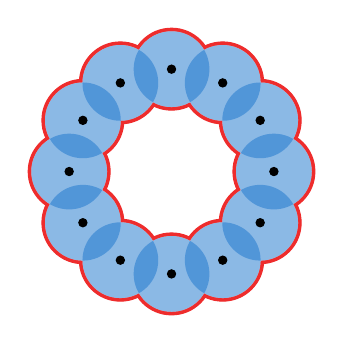
\begin{tikzpicture}[scale=1.3]
		\foreach \x in {0,30,...,330}{
			\filldraw[Firebrick2] (\x:1) circle[radius=.4];
		}
		\foreach \x in {0,30,...,330}{
			\fill[white] (\x:1) circle[radius=.37];
		}
		\foreach \x in {0,30,...,330}{
			\fill[DodgerBlue3,fill opacity=.5] (\x:1) circle[radius=.37];
			\filldraw (\x:1) circle[radius=.04];
		}
 	\end{tikzpicture}
	\caption[Unterschiede bei den Zusammenhangskomponenten zwischen $\mathcal{M}$ und $\partial \mathcal{M}$]{Angenommen die gezeichneten Entitäten bewegen sich gar nicht. Jede Niveaumenge von $\mathcal{M}$ ist dann zusammenhängend, die Niveaumengen von $\partial \mathcal{M}$ bestehen aber stets aus zwei Zusammenhangskomponenten. Da obige Konfiguration (bei geeignetem $\delta$) nur eine maximale Gruppe bildet, wurde $\mathcal{R}$ als Reeb-Graph von $\mathcal{M}$ und nicht $\partial \mathcal{M}$ definiert.}\label{fig:bsp_reeb_rand}
\end{figure}

Wie in \cref{sec:background_reeb} erläutert, entsprechen die Vertices von $\mathcal{R}$ Zeitpunkten $t_v$, an denen sich die Komponenten ändern.
Diese Zeitpunkte stimmen im Allgemeinen nicht mit den Zeitpunkten $t_0, \ldots, t_\tau$ überein, was auch in \cref{fig:tubes} zu erkennen ist.
Jeder Vertex im Reeb-Graphen lässt sich eindeutig einer der folgenden Klassen zuordnen
\begin{description}
	\item[Start-Vertex] Für jede Komponente zum Zeitpunkt $t_0$ existiert ein Vertex; ein solcher Vertex ist ein \Index{Start-Vertex}.
	Jeder Start-Vertex hat Eingangs-Grad 0 und Ausgangsgrad 1.
	\item[End-Vertex] Genauso existiert für jede Komponente zum Zeitpunkt $t_\tau$ ein Vertex, ein sog. \Index{End-Vertex}.
	Jeder End-Vertex hat Eingangs-Grad 1 und Ausgangsgrad 0.
\end{description}
Die verbleibenden Vertices können wir aufgrund der Annahme, dass keine drei Entitäten zur gleichen Zeit $\varepsilon$-(un)zusammenhängend werden, eindeutig einer der beiden folgenden Klassen zuordnen: Ein
\begin{description}
	\item[Merge-Vertex] hat Eingangs-Grad 2 und Ausgangsgrad 1, ein
	\item[Split-Vertex] hat Eingangs-Grad 1 und Ausgangsgrad 2.
\end{description}
Eine gerichtete Kante $e=(u,v)$ in $\mathcal{R}$ entspricht einer Menge von Entitäten, die zu jedem Zeitpunkt $t \in \benbrace*{t_u,t_v}$ eine Komponente (im Sinne von \cref{cha:def_gruppe}) bildet.
Wir halten fest, dass der Reeb-Graph $\mathcal{R}$ nur vom räumlichen Parameter $\varepsilon$, aber nicht von den beiden weiteren Parametern unseres Modells, $m$ und $\delta$, abhängt.

Wie genau hängt der Reeb-Graph $\mathcal{R}$ nun mit den Trajektorien und den Gruppen zusammen? 
Zunächst einmal folgt jede Entität einem Pfad in $\mathcal{R}$ von einem Start-Vertex zu einem End-Vertex.
Analog lässt sich jeder (maximalen) Gruppe ein Pfad von einem Start- oder Merge-Vertex zu einem End- oder Split-Vertex zuordnen.
Wählt man nun $m > 1$ oder $\delta > 0$, so kann es sein, dass einigen Kanten von $\mathcal{R}$ keine Gruppe zugeordnet ist und sie somit für die \GrpStruktur irrelevant sind.
$\mathcal{R}$ ohne all diese Kanten ist der \Index{reduzierte Reeb-Graph}, den wir ebenfalls mit $\mathcal{R}$ bezeichnen (nur für die Komplexität von $\mathcal{R}$ nehmen wir gleich noch einmal den unreduzierten Fall an).


\begin{definition}[{name=[{\GrpStruktur}]}]
	Die \Index{\GrpStruktur} (\enquote{trajectory grouping structure}) zu $\mathcal{X}$ und den Parametern $(\varepsilon,\delta,m)$ besteht aus dem reduzierten Reeb-Graphen $\mathcal{R}$ und einer Abbildung, die jeder Kante eine Menge maximaler Gruppen zuordnet.
\end{definition}


% section trajek_reeb (end)

\section{Komplexität der Anzahl maximaler Gruppen} % (fold)
\label{sec:max_gruppen_komplex}

% section max_gruppen_komplex (end)


% chapter reeb_graphen (end)

\chapter{Robuste Gruppen} % (fold)
\label{cha:robust}


\chapter{Related Work} % (fold)
\label{cha:related_work}
\todo[inline]{bessere Überschrift}
\todo[inline]{chronologische Reihenfolge betrachten?}
% chapter related_work (end)

% chapter robuste_gruppen (end)






\cleardoubleoddemptypage
\pagenumbering{Alph}
\setcounter{page}{1}
\appendix
\chapter{Anhang} % (fold)
\label{cha:anhang}
\section{Karte mit Niveaulinien} % (fold)
\label{sec:karte_niveau}
%!TEX root = ../trajectory-grouping.tex
In \cref{fig:zaferna} sieht man einen Kartenausschnitt von Google Maps\texttrademark{} mit aktivierter \enquote{Gelände}-Option, sodass Niveaulinen sichtbar sind.
Der Kartenausschnitt zeigt den Ort Mittelberg in Österreich.
Auch ohne die eingezeichneten Lifte könnte man anhand der Niveaulinien erkennen, dass es sich hierbei um einen Ort in einer Bergregion handelt.
\getmap[type=terrain,scale=2,zoom=13,xsize=640,ysize=400,file=zaferna,markers={}]{Mittelberg Zafernalift}
\begin{figure}[hbtp]
	\centering
	\includegraphics[width=.9\textwidth]{zaferna}
	\caption{Niveaulinien in Google Maps\texttrademark, \cite{googlemaps}}\label{fig:zaferna}
\end{figure}

% section karte_niveau (end)
% chapter anhang (end)
\printindex
\listoffigures
\printbibliography
\todototoc
\listoftodos[To-do's und andere Baustellen]
\end{document}